\documentclass[10pt]{article}
\usepackage[utf8]{inputenc}
\usepackage[T1]{fontenc}
\usepackage{amsmath}
\usepackage{amsfonts}
\usepackage{amssymb}
\usepackage[version=4]{mhchem}
\usepackage{stmaryrd}
\usepackage{graphicx}
\usepackage[export]{adjustbox}
\graphicspath{ {./images/} }

\begin{document}
Show all work as necessary. No calculators are allowed for this assessment!

\begin{enumerate}
  \item Simplify: $\sqrt[3]{200}(\sqrt[3]{135}+\sqrt[3]{40})$. (2 points)
  \item Graph $g(x)=2 \sqrt{6-x}-1$ on the axes below and use it to find the key features requested. Remember to clearly include at least 3 points on the graph of $g(x)$. (8 points)\\
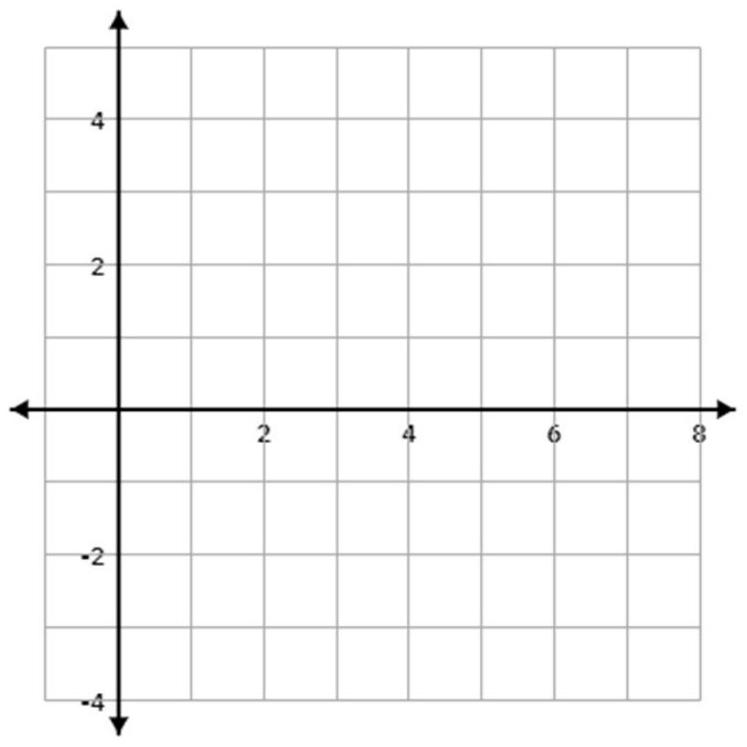
\includegraphics[max width=\textwidth, alt={}, center]{4202047f-fedd-4604-8fb5-672a0084fbd6-1_747_747_820_210}
\end{enumerate}

Domain: $\_\_\_\_$

Range: $\_\_\_\_$

Interval(s) of Increase: $\_\_\_\_$

Interval(s) of Decrease : $\_\_\_\_$

Concave Up: $\_\_\_\_$

Concave Down: $\_\_\_\_$\\
3. Which of the following BEST describes the behavior of $g(x)$ over the interval $[-27,-9]$ ? (1 point)\\
a) Increasing with a decreasing rate of change\\
b) Decreasing with an increasing rate of change\\
c) Increasing with an increasing rate of change\\
d) Decreasing with a decreasing rate of change\\
4. Solve the equation for $x$. Express all algebraic solutions. Then indicate any extraneous solutions. If there are no extraneous solutions, write "no extraneous solutions." (4 points)

$$
x-2=-2 \sqrt{x-3}
$$

\begin{enumerate}
  \setcounter{enumi}{4}
  \item Finish graphing $f(x)$ on the axes provided below. Then, identify the key features requested. All intervals MUST be expressed in interval notation (including concave up and concave down). (12 points)
\end{enumerate}

$$
f(x)= \begin{cases}-(x+3)^{2}+4 & -6 \leq x<-2 \\ 1-x & -2<x<0 \\ \sqrt{1+x}+2 & 0 \leq x<3 \\ \frac{(x+7)}{2} & 3<x \leq 5\end{cases}
$$

\begin{center}
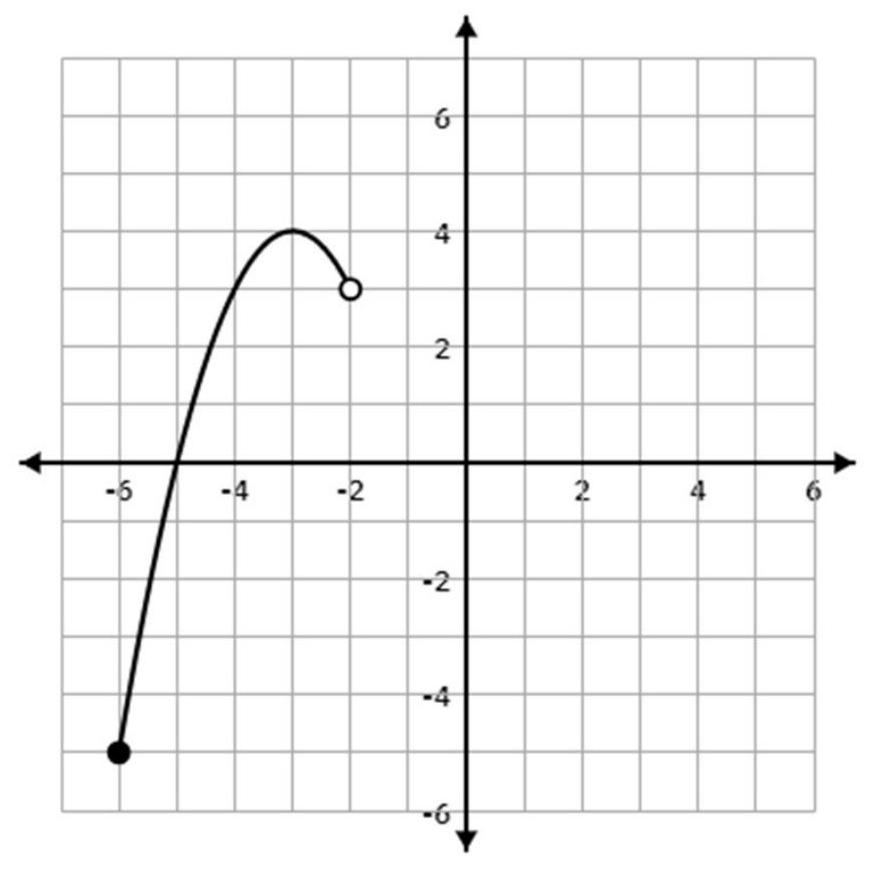
\includegraphics[max width=\textwidth, alt={}]{4202047f-fedd-4604-8fb5-672a0084fbd6-2_871_874_595_575}
\end{center}

Domain: $\_\_\_\_$

Range: $\_\_\_\_$

Interval(s) of Increase: $\_\_\_\_$

Interval(s) of Decrease: $\_\_\_\_$

Concave Up: $\_\_\_\_$

Concave Down: $\_\_\_\_$

Absolute Minimum: $\_\_\_\_$

Absolute Maximum: $\_\_\_\_$\\
$\lim _{x \rightarrow 0^{-}} f(x)=$ $\_\_\_\_$

Show all work as necessary. No calculators are allowed for this assessment!

\begin{enumerate}
  \item Simplify: $2 \sqrt[3]{32}(\sqrt[3]{16}-\sqrt[3]{54})$. (2 points)
  \item Graph $g(x)=-2 \sqrt{7-x}+2$ on the axes below and use it to find the key features requested. Remember to clearly include at least 3 points on the graph of $g(x)$. (8 points)\\
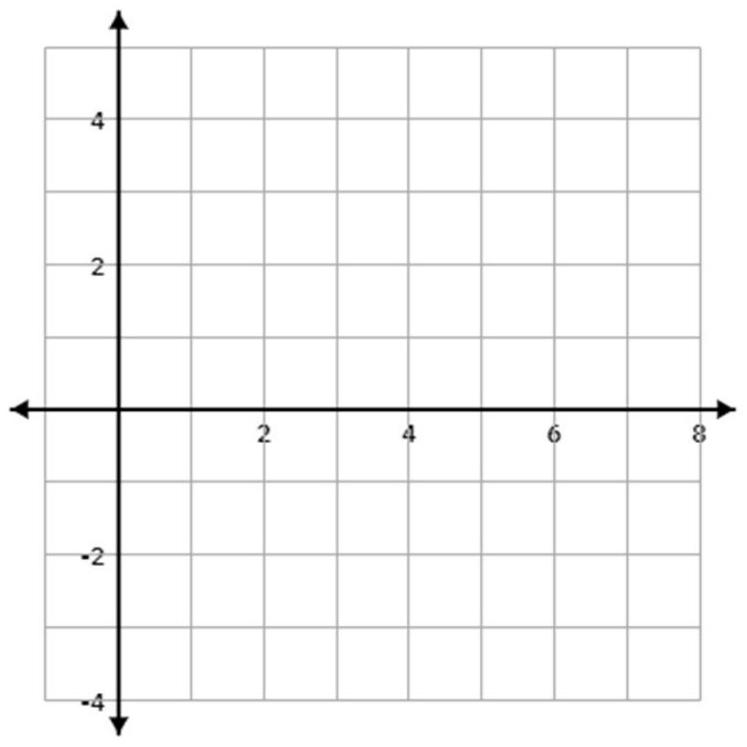
\includegraphics[max width=\textwidth, alt={}, center]{4202047f-fedd-4604-8fb5-672a0084fbd6-3_747_747_820_210}
\end{enumerate}

Domain: $\_\_\_\_$

Range: $\_\_\_\_$

Interval(s) of Increase: $\_\_\_\_$

Interval(s) of Decrease : $\_\_\_\_$

Concave Up: $\_\_\_\_$

Concave Down: $\_\_\_\_$\\
3. Which of the following BEST describes the behavior of $g(x)$ over the interval $[-9,-3]$ ? (1 point)\\
a) Increasing with a decreasing rate of change\\
b) Decreasing with an increasing rate of change\\
c) Increasing with an increasing rate of change\\
d) Decreasing with a decreasing rate of change\\
4. Solve the equation for $x$. Express all algebraic solutions. Then indicate any extraneous solutions. If there are no extraneous solutions, write "no extraneous solutions." (4 points)

$$
2-x=-2 \sqrt{5-x}
$$

\begin{enumerate}
  \setcounter{enumi}{4}
  \item Finish graphing $f(x)$ on the axes provided below. Then, identify the key features requested. All intervals MUST be expressed in interval notation (including concave up and concave down). (12 points)
\end{enumerate}

$$
f(x)= \begin{cases}(x+3)^{2}+2 & -5 \leq x<-2 \\ 1-x & -2<x<0 \\ -\sqrt{1+x}-2 & 0 \leq x<3 \\ \frac{(x-5)}{2} & 3<x \leq 5\end{cases}
$$

\begin{center}
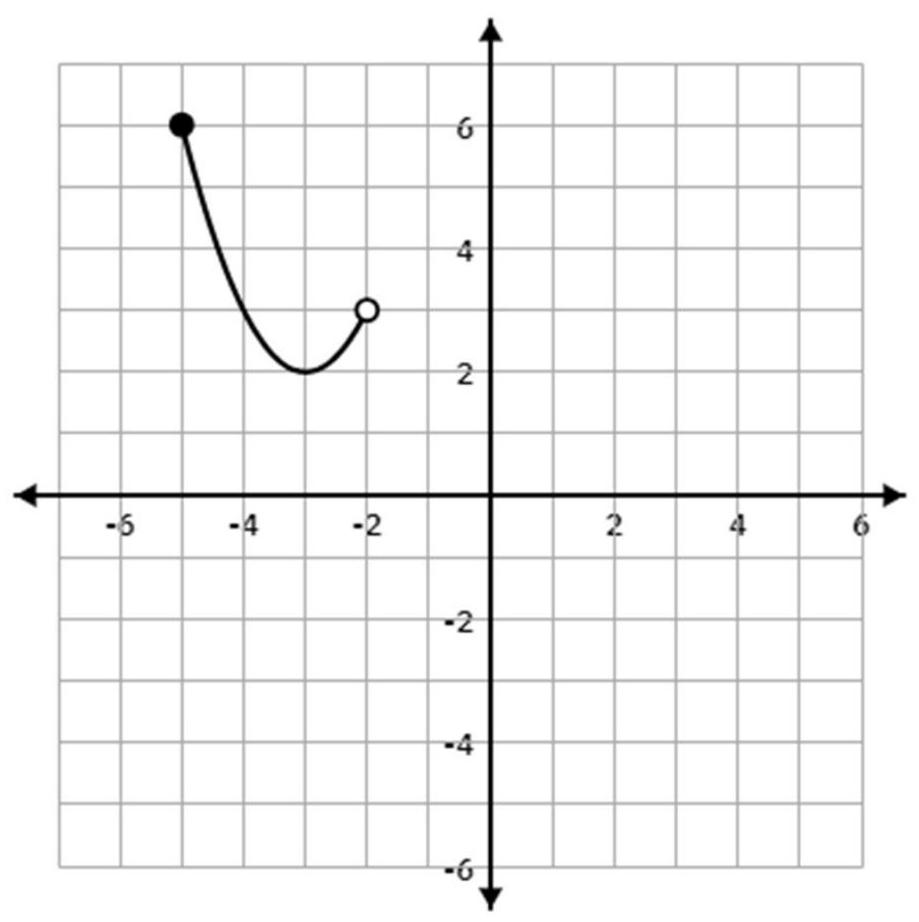
\includegraphics[max width=\textwidth, alt={}]{4202047f-fedd-4604-8fb5-672a0084fbd6-4_922_919_597_603}
\end{center}

Domain: $\_\_\_\_$

Range: $\_\_\_\_$

Interval(s) of Increase: $\_\_\_\_$

Interval(s) of Decrease: $\_\_\_\_$

Concave Up: $\_\_\_\_$

Concave Down: $\_\_\_\_$

Absolute Minimum: $\_\_\_\_$

Absolute Maximum: $\_\_\_\_$\\
$\lim _{x \rightarrow 3^{-}} f(x)=$ $\_\_\_\_$

Show all work as necessary. No calculators are allowed for this assessment!

\begin{enumerate}
  \item Simplify: $2 \sqrt[3]{250}(\sqrt[3]{32}-\sqrt[3]{108})$. (2 points)
  \item Graph $g(x)=2 \sqrt{4-x}-2$ on the axes below and use it to find the key features requested. Remember to clearly include at least 3 points on the graph of $g(x)$. (8 points)\\
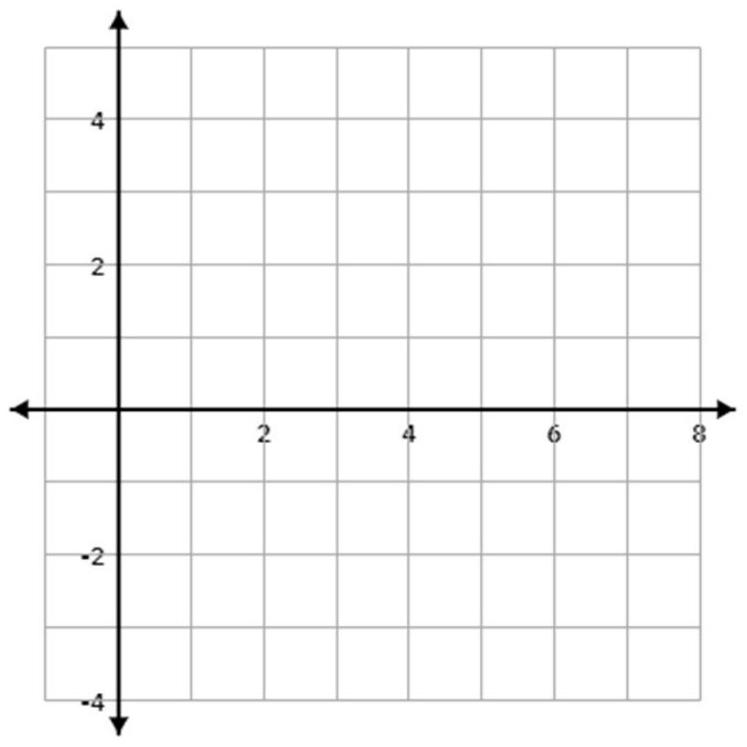
\includegraphics[max width=\textwidth, alt={}, center]{4202047f-fedd-4604-8fb5-672a0084fbd6-5_747_747_820_210}
\end{enumerate}

Domain: $\_\_\_\_$

Range: $\_\_\_\_$

Interval(s) of Increase: $\_\_\_\_$

Interval(s) of Decrease : $\_\_\_\_$

Concave Up: $\_\_\_\_$

Concave Down: $\_\_\_\_$\\
3. Which of the following BEST describes the behavior of $g(x)$ over the interval $[-19,-9]$ ? (1 point)\\
a) Increasing with a decreasing rate of change\\
b) Decreasing with an increasing rate of change\\
c) Increasing with an increasing rate of change\\
d) Decreasing with a decreasing rate of change\\
4. Solve the equation for $x$. Express all algebraic solutions. Then indicate any extraneous solutions. If there are no extraneous solutions, write "no extraneous solutions." (4 points)

$$
3-x=-2 \sqrt{x-3}
$$

\begin{enumerate}
  \setcounter{enumi}{4}
  \item Finish graphing $f(x)$ on the axes provided below. Then, identify the key features requested. All intervals MUST be expressed in interval notation (including concave up and concave down). (12 points)
\end{enumerate}

$$
f(x)= \begin{cases}(x+3)^{2}-2 & -4<x \leq-1 \\ -x+4 & -1<x<1 \\ -\sqrt{x-1}-2 & 1<x \leq 5 \\ \frac{(x-5)}{2}+1 & 5<x \leq 7\end{cases}
$$

\begin{center}
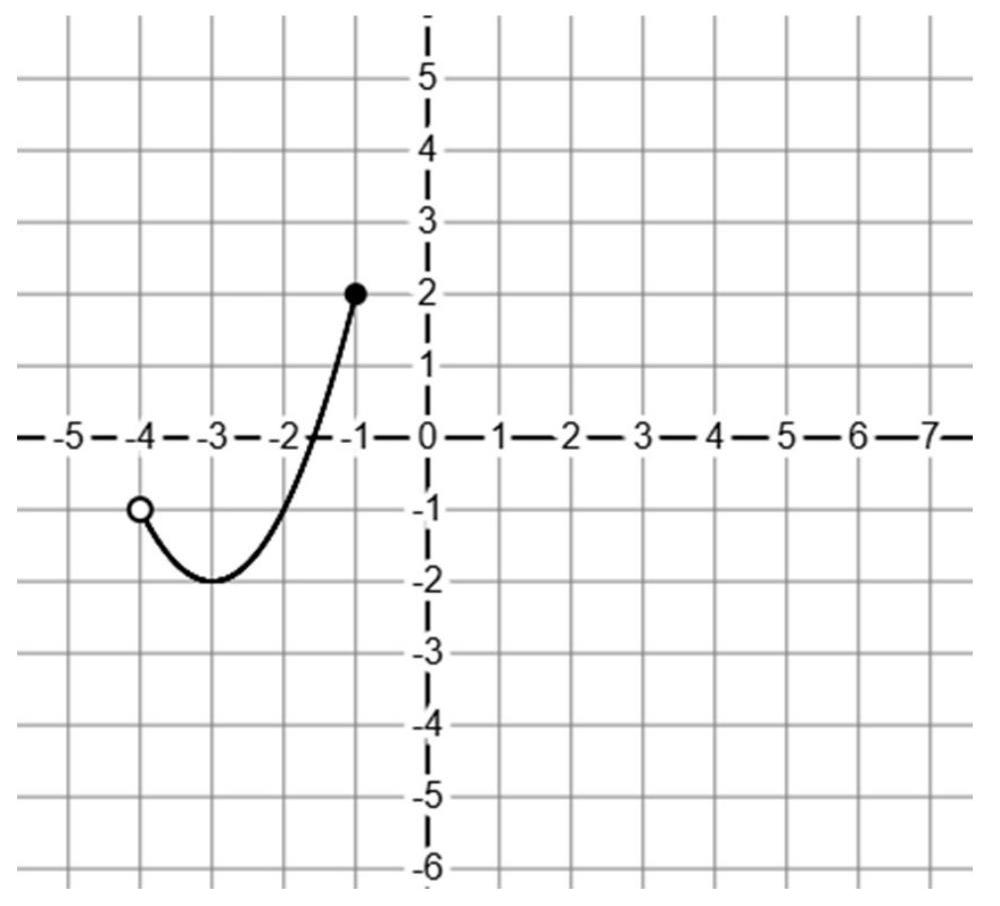
\includegraphics[max width=\textwidth, alt={}]{4202047f-fedd-4604-8fb5-672a0084fbd6-6_906_1000_575_504}
\end{center}

Domain: $\_\_\_\_$

Range: $\_\_\_\_$

Interval(s) of Increase: $\_\_\_\_$

Interval(s) of Decrease: $\_\_\_\_$

Concave Up: $\_\_\_\_$

Concave Down: $\_\_\_\_$

Absolute Minimum: $\_\_\_\_$

Absolute Maximum: $\_\_\_\_$\\
$\lim _{x \rightarrow 5^{+}} f(x)=$ $\_\_\_\_$


\end{document}